\section{Data Description \& Analysis}
\label{sec:3_data}
% approx. 200-500 words
\paragraph*{Description}
The dataset used to train and evaluate the model is word-level Penn Treebank\cite{marcus1993building}, which is a variation of the original Penn Treebank dataset built to be best suited to language modelling settings. 

Specifically, the original Penn Treebank has undergone a pre-processing pipeline so that it features:

\begin{itemize}
    \item consistent lowercase;
    \item tokenization;
    \item no punctuation;
    \item proper nouns and other rare words have been encompassed by a \texttt{<unk>} token;
    \item digits have been replaced with a \texttt{N} token;
    \item no OOV words in \emph{validation} and \emph{test} sets with respect to the \emph{training} set.
\end{itemize}

\begin{table}
    \begin{tabular}{lccc}
    \toprule
    & \textbf{Train} & \textbf{Validation} & \textbf{Test} \\
    \midrule
    Sents split percentage & 
    \(85.51\)\% & \(6.85\)\% & \(7.64\)\%  \\
    Words split percentage & 
    \(85.62\)\% & \(6.79\)\% & \(7.59\)\%  \\
    \# Sentences & 
    \(42,068\) & \(3,370\) & \(3,761\) \\
    \# Words & 
    \(887,521\) & \(70,390\) & \(78,669\) \\ 
    \# Vocabulary & 
    \(9,999\) & \(6,021\) & \(6,048\) \\
    \# OOV words & 
    - & \(0\) & \(0\) \\
    \midrule
    Sentence lengths mean & 
    \(20.09\) & \(20.88\) & \(20.91\) \\
    Sentence lengths median & 
    \(20.0\) & \(20.0\) & \(20.0\) \\
    Sentence lengths \(\sigma\) &
    \(10.14\) & \(9.98\) & \(10.18\) \\
    Sentence max length & 
    \(82\) & \(74\) & \(77\) \\
    Sentence min length & 
    \(1\) & \(1\) & \(1\) \\

    \bottomrule
\end{tabular}
    \caption{Statistics of word-level Penn Treebank}
    \label{tab:statistics}
\end{table}

\paragraph*{Statistics analysis}
In Tab.\ref{tab:statistics} we are presenting a summary of the relevant statistics of the dataset.

The PTB dataset appears to be balanced enough, as sents and words are evenly splitted and the mean and standard deviance \(\sigma\) of the words-per-sentence distribution are very similar, being around \(20\) and \(10\).

Moreover, since there are no OOV words, we can rely on the train split to construct the vocabulary. Its length is given by the \(9999\) words, to which we added two additional tokens:
\begin{itemize}
    \item \texttt{<pad>} is a pad token to pad shorter sequences to the length of the longest sequence in a given batch;
    \item \texttt{<eos>} is a sentence terminator token.
\end{itemize}

The analysis of the most frequent words in the train split reveals that the most frequent words are extremely common function words, like articles (\textit{the}, \(5.7\)\%), or prepositions (\textit{of}, \(2.7\)\%), which is unsurprising. We are not surprised to observe that the two wrappers \texttt{<unk>} and \texttt{N} show high counts, being \(5.1\)\% and \(3.7\)\% respectively, ranking second and third most frequent words. Ultimately, the first 10 most frequent words make up almost 30\% of the total word count.

\begin{figure}[!t]
    \centering
    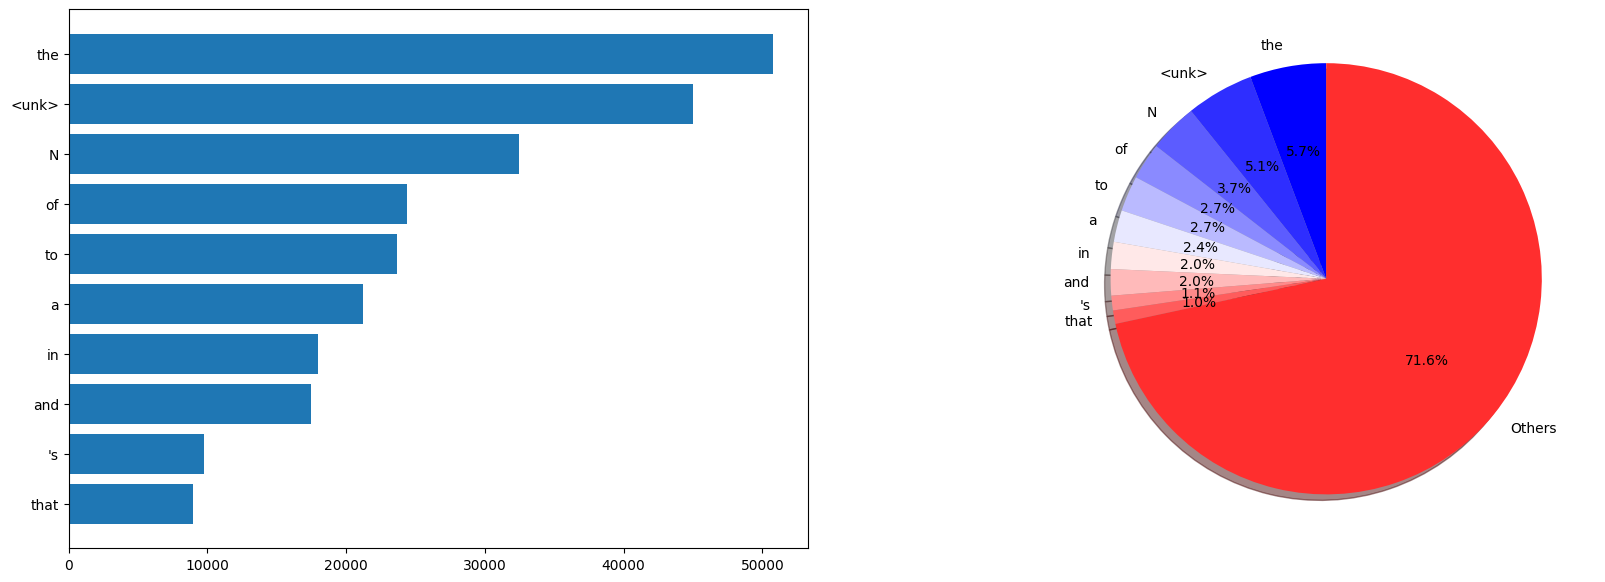
\includegraphics[keepaspectratio,width=.5\textwidth]{assets/images/train_freq.png}
    \caption{Frequency distribution of the 10 most frequent words (Train)} 
    \label{fig:train_freq}
\end{figure}
